\section{Generel beskrivelse}

\subsection{Systembeskrivelse}

\begin{itemize}

\item Brugersystem \\
Brugersystemet st�r til ansvar for, at brugeren f�r en intuitiv indgang til systemet. Dette system d�kker hele brugeroplevelsen, herunder at kunne v�lge en busrute og se denne p� kortet. Brugersystemet d�kker intet administrativt, og brugeren skal ikke have nogen specielle evner for at bruge denne del af systemet.

\item Administrations system  \\ 
Administrations systemet st�r til ansvar for, at administratoren kan �ndre persisteret data nemt, uden at skulle tilg� databasen direkte. Dette systeme d�kker over en r�kke v�rkt�jer som kan manipulere data for busser og deres ruter. Systemet har ingen p�virkning p� brugersystemet, ud over de �ndringer der sker p� persisteret data.

\item Positionsdata \\
Positionsdata, er infomrationen om bussens placering. Position persisteres direkte, uden om administrations systemet og brugersystemet. Denne del kan simuleres uden tab af funktionalitet.

\item Distribueret persisteret data \\
Persisteret data er kerneelementet i dette projekt. Persisteret data er to-delt og best�r i den globale persisterede data og lokalt persisteret data. Globalt persisteret data vil best� af alt den information brugersystemet og administrations systemet har til f�lles, hvor et eksempel kunne v�re positionsdata. Lokalt persisteret data vil best� af den information brugeren har valgt at gemme lokalt fra brugersystemet, dette vil prim�rt best� af favoriserede busruter. 

\item Lokalt Distribueret data
\end{itemize}

\begin{figure}[u]
\centering
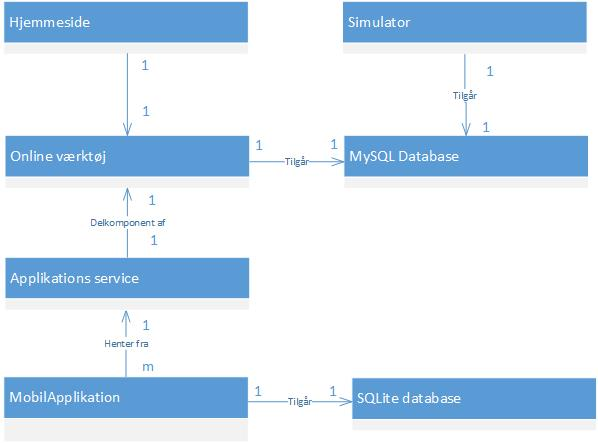
\includegraphics[scale=0.7]{Domainmodel_Billede.jpg}
\caption{Dom�nemodel}
\label{domainmodel}
\end{figure} 

p� figur \ref{domainmodel} gives der et overblik over systemet, hvor enhederne ses i sammenh�ng. De forskellige enheder er beskrevet kort i ovenst�ende afsnit, \emph{2.1 Systembeskrivelse}. Diagramet er lavet med online-v�rk�jet creately.com.

%\subsubsection{Akt�r kontekst-diagram}

\begin{figure}[h]
\centering
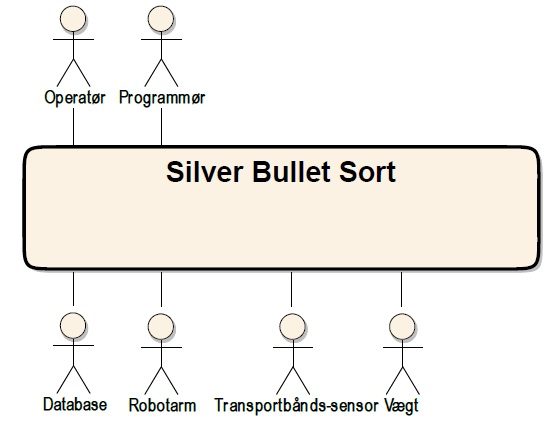
\includegraphics[scale=0.5]{Andet/AktOr-kontekst.jpg}
\caption{Akt�r kontekst-diagram}
\end{figure}

Ovenst�ende figur viser hvilke akt�rer, der interagerer med sorteringssystemet. Videre beskrivelse af disse akt�rer, findes i f�lgende afsnit \emph{2.1.3 Akt�rbeskrivelser}  
\newpage

%\subsubsection{Akt�r beskrivelse}

\underline{\textbf{Prim�re akt�rer:}}\\
\begin{tabular}{lp{10 cm}}

\textbf{Akt�r navn} 				& Operat�r\\
\textbf{Beskrivelse} 				& Denne akt�r starter og stopper systemet. M�let for akt�ren er at f� sorteret klodser, alt efter deres materialetype. \\
\textbf{Antal samtidige akt�rer}	& 1 \\
\\\\
\textbf{Akt�r navn}					&  Programm�r. \\ 
\textbf{Beskrivelse} 				&  Denne akt�rs opgave er at lave brugerdefinerede programmer til systemet.\\ 
\textbf{Antal samtidige akt�rer} 	&  1
\end{tabular}
\\\\
\\\\
\underline{\textbf{Sekund�re akt�rer}}
\\
\begin{tabular}{lp{10 cm}}

\textbf{Akt�r navn} 				& V�gt\\
\textbf{Beskrivelse} 				& Denne akt�r vejer et objekt, s� systemet kan bestemme dets materialetype.  \\
\textbf{Antal samtidige akt�rer}	& 1 \\
\\\\
\textbf{Akt�r navn}					& Transportb�ndssensor \\
\textbf{Beskrivelse}				& Denne akt�r registrerer, hvorn�r et objekt er klar til at blive samlet op af robotten.  \\
\textbf{Antal samtidige akt�rer}	& 1 \\
\\\\
\textbf{Akt�r navn} 				&  Robotarm.\\ 
\textbf{Beskrivelse} 				&  Denne akt�rs opgave er at flytte og m�le forskellige typer klodser.\\ 
\textbf{Antal samtidige akt�rer} 	&  1 \\ 
\\\\
\textbf{Akt�r navn} 				&  Database. \\ 
\textbf{Beskrivelse} 				&  Databasen indeholder logfiler for systemets data for de enkelte klodser, samt informationer om robotten og systemets status. Ligeledes indeholder databasen programmerne, som programm�ren har lavet.\\ 
\textbf{Antal samtidige akt�rer} 	&  1
\end{tabular} 
